
\section{Thursday, May 9}

\todaybox{Finish complex division. Then, discuss rectangular and polar coordinates.}

Last class, we left off with a lemma, on the road to defining division:

\begin{manuallemma}{1.1} Let $a+bi\in \C$ be non-zero (i.e., at least one of $a,b$ is not 0). Then $\frac{1}{z} = \frac{a}{a^2 + b^2} - \frac{b}{a^2 + b^2}i$. Another way of writing this is that $\frac{1}{z} = \frac{\overline{z}}{\left|z\right|^2}$, where we understand that division by a real number means division on both the real part and imaginary part.\end{manuallemma}

\begin{proof} To show that $\frac{1}{z}$ is what we claim, we need only check that $z\frac{1}{z} = 1$. We compute:

\begin{align*}(a+bi)\left(\frac{a}{a^2 + b^2} - \frac{b}{a^2 + b^2}i\right) &= \frac{a^2 -(b)(-b)}{a^2 + b^2} + \frac{ab + a(-b)}{a^2 + b^2}i\\
&= \frac{a^2 + b^2}{a^2 + b^2}\\
&= 1\end{align*}

\end{proof}

Where did this come from? The intuition comes from the calculation:

$$\frac{1}{a+bi}{\frac{a-bi}{a-bi}} = \frac{a-bi}{(a-bi)(a+bi)} = \frac{a-bi}{a^2 + b^2}$$

We can't use this as a proof of the result, since it relies on being able to divide by complex numbers (which we haven't even defined yet!), as well as being able to manipulate fractions. However, as far as intuition goes, this is a good way to understand the result.

\begin{note} This calculation also shows that $z\OL{z} = |z|^2$. This is a very important fact, and will come up very frequently.\end{note}


This lemma lets us define division properly:

\begin{defbo}{Division}{division}\index{Algebra!division} 
Let $z,w\in \C$ with $w\ne 0$. Then:
$$\frac{z}{w} = \frac{z\overline{w}}{|w|^2}$$
\end{defbo}


\begin{ex}{}{} Let $z = 4 + 3i$ and $w = 1 + i$. Find $\frac{z}{w}$ and $\frac{w}{z}$.

We know from our formula that $\frac{z}{w} = \frac{z\overline{w}}{|w|^2}$. So we compute:
$$\overline{w} = 1 - i$$
$$|w|^2 = (1^2 + 1^2)  = 2$$
So, $\frac{z}{w} = \frac{(4 + 3i)(1 - i)}{2} = \frac{7}{2} -\frac{1}{2}i$.


To compute $\frac{w}{z}$, we could go through the same process. Or, we could note that $\frac{w}{z} = \frac{1}{\left(\frac{z}{w}\right)} = \frac{2}{7 - i}$. We then get that:

$$\frac{w}{z} = \frac{2(7+i)}{|7-i|^2} = \frac{14}{50} + \frac{2}{50}i$$

\end{ex}

How do complex conjugation and the modulus behave when combined with our algebraic operations?

\begin{thmbo}{Algebraic Properties of Conjugation and the Modulus}{conjprop}Let $z,w \in \C$.

\begin{enumerate}
\item $\OL{zw} = \OL{z}\,\OL{w}$
\item $\OL{z + w} = \OL{z} + \OL{w}$
\item $\OL{\OL{z}} = z$.
\item $z + \OL{z} = 2\RE(z)$ and $z - \OL{z} = 2\IM(z)i$.
\item $\OL{\left(\frac{z}{w}\right)} = \frac{\OL{z}}{\OL{w}}$
\item $|zw| = |z||w|$
\item $|\OL{z}| = |z|$
\item If $z = x + iy$, then $|x| \le |z|$ and $|y| \le |z|$.
\item The {\bf triangle inequality}: $|z + w| \le |z| + |w|$. And $|z + w| = |z| + |w|$ if and only if $z = rw$ for some $r\in \R$ or $w = rz$ for some $r\in \R$.
\item $\left|\frac{z}{w}\right| = \frac{|z|}{|w|}$
\end{enumerate}

\end{thmbo}

\begin{proof} We will prove some, but not all of these statements. Many of them are variations on the same idea, and so will be quick to verify.

Let $z = a+ bi$ and $w = c + di$.

\begin{enumerate}
\item From the definition, $zw = ac -bd + (ad + bc)i$. Therefore, 

$$\OL{zw} = (ac - bd) - (ad + bc)i$$

On the other hand, we find that:

$$\OL{z}\,\OL{w} = (a-bi)(c-di) = (ac - (-b)(-d)) + (a(-d) + (-b)c)i = (ac - bd) - (ad +bc)i$$

So we see that $\OL{zw} = \OL{z}\,\OL{w}$.

\setcounter{enumi}{3}

\item We have $z + \OL{z} = a + bi + (a-bi) = 2a = 2\RE(z)$, and $z - \OL{z} = (a + bi) - (a-bi) = 2bi = 2\IM(z)i$.

\setcounter{enumi}{7}

\item  Note that $|x| = \sqrt{x^2} \le \sqrt{x^2 + y^2}$, since $f(x) =\sqrt{x}$ is an increasing function on $[0,\infty)$ and $y^2\ge 0$. This shows that $|x| \le |z|$. A similar argument shows that $|y| \le |z|$.

\item To show this, it is enough to show that $|z+w|^2 \le (|z| + |w|)^2$. It will take us a bit of work to get there though.

%
%
%First, note that $(|z| + |w|)^2 = |z|^2 + 2|z||w| + |w|^2 = $. 
%
%On the other hand:
%
%\begin{align*}|z + w|^2 &= (z + w)(\OL{z} + \OL{w}) \\
%&= z\OL{z} + (z\OL{w} + \OL{z}w) + w\OL{w} \\
%&= |z|^2 + (z\OL{w} + \OL{z\OL{w}}) + |w|^2\\
%&= |z|^2 + 2\RE(z\OL{w}) + |w|^2
%\end{align*}
%
%So, we have $|z +w|^2 = |z|^2 + 2\RE(z\OL{w}) + |w|^2 \le |z|^2 + 2|z\OL{w}| + |w|^2= |z|^2 + 2|z||w| + |w|^2 = (|z| + |w|)^2$. Taking square roots of both sides gives the desired inequality.
%
%From this calculation, notice that $|z + w| = |z| + |w|$ if and only if $2\RE(z\OL{w}) = 2|z||w|$. Therefore, this occurs precisely when $ac + bd = \sqrt{a^2 + b^2}\sqrt{c^2 + d^2}$.
%
%
%
%
%
%
%




First, notice that $(ad - bc)^2 \ge 0$. This implies that

$$2abcd \le a^2d^2 + b^2c^2$$

Adding $a^2c^2 + b^2d^2$ to both sides tells us that:

$$(ac + bd)^2 \le (a^2 + b^2)(c^2 + d^2)$$

As such, it follows that $2(ac + bd) \le 2\sqrt{(a^2 + b^2)(c^2 + d^2)}$. Now, adding $a^2 + b^2 + c^2 + d^2$ to both sides gives:

$$(a^2 + 2ac + c^2) + (b^2 + 2bd + d^2) \le (a^2 + b^2) + 2\sqrt{(a^2 + b^2)(c^2 + d^2)} + (c^2 + d^2)$$

Factoring each side gives:

$$(a+c)^2 + (b+d)^2 \le (\sqrt{a^2 + b^2} + \sqrt{c^2 + d^2})^2$$

However, $(a+c)^2 + (b+d)^2 = |z+w|^2$, $\sqrt{a^2 + b^2}= |z|$, and $\sqrt{c^2 + d^2} = |w|$. So we have shown that $|z+w|^2 \le (|z|  +|w|)^2$. Taking the square root of both sides gives $|z +w| \le |z| + |w|$.


For equality, note that if $z = rw$ or $w = rz$ (and you do need either condition, since you could have $z = 0$ or $w = 0$), then $ad - bc = 0$. In that case:

$$2abcd = a^2d^2 + b^2c^2$$

And rather than having $\le$ in our calculations above, equality follows through.

\begin{note}Fisher has a shorter proof of this fact in section 1.2. However, he does not discuss equality.\end{note}


\item To begin, let's show that $\left|\frac{1}{w}\right| = \frac{1}{|w|}$. Notice that $\frac{1}{w} = \frac{c}{c^2 + d^2} - \frac{d}{c^2 + d^2}i$. And so:

\begin{align*}\left|\frac{1}{w}\right| &= \sqrt{\left(\frac{c^2}{(c^2 + d^2)^2} + \frac{d^2}{(c^2 + d^2)^2}\right)} \\
&= \sqrt{\frac{1}{c^2 + d^2}}\\
&= \frac{1}{\sqrt{c^2 + d^2}}\\
&= \frac{1}{|w|}
\end{align*}

Now, by the first result of this theorem, we see that:

$$\left|\frac{z}{w}\right| = |z|\left|\frac{1}{w}\right| = |z|\frac{1}{|w|} = \frac{|z|}{|w|}$$

\end{enumerate}

\end{proof}


\subsection{Rectangular Coordinates and $\R^2$}

One way of visualizing complex numbers is to picture them as a vector in $\R^2$.

\begin{ex}{}{} Consider $z = 3 + 2i$. Then we can visualize $z$ as the vector:

\begin{center}
\begin{tikzpicture}
%\draw [help lines,black!20!white] (-1,-1) grid (4,4);
\foreach \x in {-1,1,2,3}
       \draw[xshift=\x cm, thick] (0pt,-1pt)--(0pt,1pt) node[below] {$\x$};
\foreach \y in {-1,1,2,3}
       \draw[yshift=\y cm, thick] (-1pt,0pt)--(1pt,0pt) node[left] {$\y$};    

\draw[thick] (0,-1) -- (0,3);
\draw[thick] (-1,0) -- (3,0);

\draw[->] (0,0) -- (3,2);

\draw (3,2) node[above]{$z$}; 

\end{tikzpicture}
\end{center}

\end{ex}

\begin{note} In general, we can visualize the complex number $z = x + iy$ as the point $(x,y)$ on the plane.

However, this does not mean that $\C$ and $\R^2$ are the same thing. They are not. We cannot multiply vectors in $\R^2$. We can't divide by vectors. Etc.
\end{note}

\begin{defbo}{Rectangular Coordinates}{rectCoords} \index{Coordinates!rectangular} The {\bf rectangular coordinates} of $z \in \C$ is the point $(\RE(z), \IM(z))$ in $\R^2$.

When we write $z = x + iy$, we say that $z$ is written in {\bf rectangular form}.
\end{defbo}


This perspective does allow us to give some fairly nice proofs. For example:

\begin{thmbo}{The Triangle Inequality}{triangIneq}
 Let $z = x+iy$. Then $|z|$ is equal to the length of the vector $(x,y)$.

\vspace{5pt}

As a consequence, $|z + w| \le |z| + |w|$.
\end{thmbo}

\begin{proof} The first claim is fairly straightforward: $|z| = \sqrt{x^2 + y^2}$, and the length of the vector $(x,y)$ is $\lVert (x,y) \rVert = \sqrt{x^2 + y^2}$.

So, let $w,z\in \C$ and let $\vec{w}$ and $\vec{z}$ be their corresponding vectors in $\R^2$. Now, consider the following picture:

\begin{center}
\begin{tikzpicture}

\draw[thick] (0,-2) -- (0,3);
\draw[thick] (-2,0) -- (3,0);


\node at (0,0) (origin){};
\node at (1,2) (z){};
\node at (2,-1) (sum){};

\draw[->] (origin) -- (z) node [midway, left]{$\vec{z}$};

\draw[->, red] (z)-- (sum) node [midway, right]{$\vec{w}$};

\draw[->, blue] (origin) -- (sum) node [inner sep = 9pt, midway, below]{$\vec{z} + \vec{w}$};

\end{tikzpicture}
\end{center}

The vectors $\vec{z}$,  $\vec{w}$, and $\vec{z} + \vec{w}$ satisfy the triangle inequality: $\lVert \vec{z} + \vec{w} \rVert \le \lVert\vec{z}\rVert + \lVert\vec{w}\rVert$. And further, equality occurs precisely when $\vec{z}$ and $\vec{w}$ are in the same direction.

However, since the lengths of these vectors are equal to the corresponding moduli of the complex numbers, we conclude the triangle inequality on $\C$.

\end{proof}

\subsection{Polar Coordinates}

Let $z = x + iy$. We have seen that there is one way to represent complex numbers visually, via rectangular coordinates. There is another, which is in many ways much more important. Consider the picture:

\begin{center}
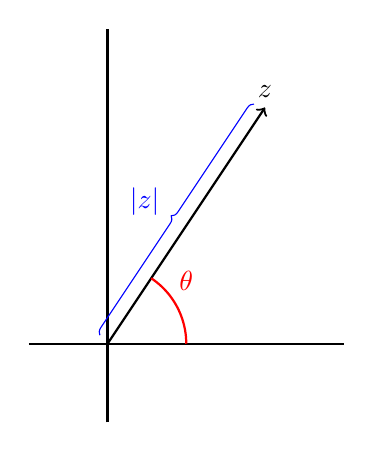
\begin{tikzpicture}
%\draw [help lines,black!20!white] (-1,-1) grid (4,4);

\draw[thick] (0,-1) -- (0,4);
\draw[thick] (-1,0) -- (3,0);

\draw[thick, ->] (0,0) -- (1.2,1.8) node [blue, inner sep = 15pt, left]{$|z|$} -- (2,3);
\draw[blue, decorate, decoration = {brace, raise = 4pt}] (0.02,0.03)--(1.98,2.97);

\draw (2,3) node[above]{$z$}; 

\draw [red,thick,domain=0:56.3] plot ({cos(\x)}, {sin(\x)});

\draw (1, 0.8) node [red] {$\theta$};

\end{tikzpicture}
\end{center}

We can also express this vector in $\R^2$ by giving its length, $|z|$, and the angle it forms with the positive $x$-axis, $\theta$.

\begin{lem} If $z\in \C$ with $|z| = r$, and $z$ forms an angle of $\theta$ with the positive $x$-axis, then:

$$z = r(\cos(\theta) + i\sin(\theta))$$
\end{lem}

\begin{proof} Suppose $|z| = r$. Then the vector $\vec{z}$ in $\R^2$ has $\lVert \vec{z}\rVert = r$. As such, $\vec{z}$ is on a circle of radius $r$, which we know (from MAT235) is parametrized by the equations $x = r\cos(\theta)$ and $y = r\sin(\theta)$, where $\theta$ is the angle between $\vec{z}$ and the positive $x$-axis.

As such, we conclude that $z = x + iy = (r\cos(\theta)) + (r\sin(\theta))i$, as desired.
\end{proof}


\begin{defbo}{Polar Coordinates}{polarCoords}\index{Coordinates!polar}
 Let $z\in \C$. Then we say that $z$ is in {\bf polar coordinates}, or in {\bf polar form}, if we write $z$ as $z = r(\cos(\theta) + i\sin(\theta))$.

In this expression, $r = |z|$ and $\theta$ is the angle between $z$ and the positive $x$-axis.
\end{defbo}

\begin{ex}{}{} Find the real and imaginary parts of $z = 2(\cos(0.2) + i\sin(0.2))$.

Well, $z = 2\cos(0.2) + (2\sin(0.2))i$, and so $\RE(z) = 2\cos(0.2)$ and $\IM(z) = 2\sin(0.2)$.

\end{ex}

\begin{note} Be careful! The real part of $z$ is not $2$. $2$ is its modulus! This is a very common mistake!\end{note}


\begin{ex}{}{} Write $|z| = 4 - 4\sqrt{3}i$ in polar form.

Let's start by finding $|z|$. This is always easier. We compute: $|z| = \sqrt{16 + (16)(3)} = \sqrt{64} = 8$.

Now, we can see that $z$ forms a right angle triangle with the positive real axis which has hypotenus $8$, and side lengths $4$ and $4\sqrt{3}$. If we view this as:

\begin{center}
\begin{tikzpicture}
%\draw [help lines,black!20!white] (-1,-1) grid (4,4);

\draw[thick] (0,-4) -- (0,1);
\draw[thick] (-1,0) -- (3,0);

\draw[->] (0,0) -- (2,-3);

\draw (2,-3) node[below]{$z$}; 

\draw [red,thick,domain=0:-56.3] plot ({cos(\x)}, {sin(\x)});

\draw (1, -0.8) node {$\Psi$};

\end{tikzpicture}
\end{center}

Then we have that $\Psi = -\theta$ and that:
\begin{align*} \cos\Psi &= \frac{4}{8} = \frac{1}{2}\\
\sin(\Psi) &= \frac{4\sqrt{3}}{8} = \frac{\sqrt{3}}{2}
\end{align*}

We know from our special triangles that this gives $\Psi = \frac{\pi}{3}$. Therefore, $\theta = -\frac{\pi}{3}$.

So, in polar form, we have $4 - 4\sqrt{3}i = 8\left(\cos\left(\frac{-\pi}{3}\right) + i\sin\left(\frac{-\pi}{3}\right)\right)$.

\end{ex}

There is another bit of notation, which you may have come across, used to write polar form.

\begin{defbo}{Euler's Formula}{eulerForm}\index{Euler's Formula} 
$e^{i\theta} = \cos(\theta) + i\sin(\theta)$.
\end{defbo}

So, instead of writing $z = r(\cos(\theta) + i\sin(\theta))$, we will from now on write $z = re^{i\theta}$. We will discuss why we use this notation (why $e$?), later on in the course. There is a reason.

\begin{ex}{}{} Find the polar form for $z = \frac{-1}{\sqrt{2}} + \frac{1}{\sqrt{2}}i$, and write it as $z = re^{i\theta}$.

We know that $r = |z|$. So we compute:
$$|z| = \sqrt{\left(\frac{-1}{\sqrt{2}}\right)^2 + \left(\frac{1}{\sqrt{2}}\right)^2} = \sqrt{1} = 1$$

As for the angle, we need to be careful here. If we were to take the angle $\theta = \arctan\left(\frac{y}{x}\right) = \arctan(-1)$, we would end up with an angle in the fourth quadrant. But our complex number is in the second quadrant. So how do we handle this?

Well, note that our angle $\theta$ and $\arctan(1)$ are on directly opposite sides of the unit circle, and so $\theta = \arctan(-1) + \pi = \frac{3 \pi}{4}$.

Therefore, $z = 1e^{i\frac{3\pi}{4}}$.

\end{ex}

\begin{ex}{}{} True or false: the real part of $3e^{i\frac{\pi}{2}}$ is $3$.

False. This is a mistake I saw quite a lot last summer. You need to be able to find the real and imaginary parts of a complex number written in polar form.

In this case, $3e^{i\frac{\pi}{2}} = 3\left(\cos\left(\frac{\pi}{2}\right) + i\sin\left(\frac{\pi}{2}\right)\right) = 3(0 + i) = 3i$. So the real part of this complex number is 0!

\end{ex}

Polar coordinates are useful in a variety of ways, which are majorly different from the ways in which rectangular form is useful. One way is that working in polar form makes doing multiplication very easy.

\begin{thmbo}{Multiplication in Polar Form}{polarmult} \index{Algebra!multiplication in polar form}
 Let $z = re^{i\theta}$ and $w = Re^{i\Psi}$. Then:
$$zw = rRe^{i(\theta + \Psi)}$$
\end{thmbo}

\begin{proof} We go back to rectangular coordinates. $z = r(\cos(\theta) + i\sin(\theta))$ and $w = R(\cos(\Psi) + i\sin(\Psi))$. Then:

\begin{align*} zw =& rR(\cos(\theta) + i\sin(\theta))(\cos(\Psi) + i\sin(\Psi))\\
=& rR\left(\left[\cos(\theta)\cos(\Psi) - \sin(\theta)\sin(\Psi)\right]\right.\\
& +\left. i\left[\sin(\theta)\cos(\Psi) + \cos(\theta)\sin(\Psi)\right]\right)\\
=&rR(\cos(\theta + \Psi) + i\sin(\theta + \Psi) \qquad\qquad (\text{trig identities})\\
=&rRe^{i(\theta + \Psi)}
\end{align*}

\end{proof}

A similar argument can also be used to prove: 

\begin{thmbo}{Division in Polar Form}{polarDiv} \index{Algebra!division in polar form}
 Let $z = re^{i\theta}$ and $w = Re^{i\Psi}\ne 0$. Then:
$$\frac{z}{w} = \frac{r}{R}e^{i(\theta - \Psi)}$$
\end{thmbo}

\begin{proof} The proof is similar to that of theorem \ref{thm:polarmult}, except using the angle difference formulas for $\sin$ and $\cos$. Consider working through the proof, mimicing the proof of theorem \ref{thm:polarmult}.\end{proof}

\begin{note} The key ingredients in these proofs are trig identities. Specifically, the angle sum (and angle difference) formulas. Trig is very important to working with complex numers. You will need to know your trig identities. \end{note}

Since multiplying in polar form is very quick, taking powers should also be really quick. Intuitively, the argument above tells us that if $\theta$ is an angle for $z$, then $n\theta$ is an angle for $z^n$. After all, if we add $n$ copies of $\theta$, we get $n\theta$. This intuitive idea is actually a named theorem!

\begin{thmbo}{De Moivre's Theorem}{demoivre} \index{De Moivre's Theorem}
Let $n\in \N$. Then $(\cos(\theta) + i\sin(\theta))^n = \cos(n\theta) + i\sin(n\theta)$.
\end{thmbo}

\begin{proof} We proceed by induction. The claim is clearly true for $n = 1$.

Suppose $(\cos(\theta) + i\sin(\theta))^n = \cos(n\theta) + i\sin(n\theta)$. This really just says: $(e^{i\theta})^n = e^{i(n\theta)}$.

Now, consider $(\cos(\theta) + i\sin(\theta))^{n+1}$. We have:

\begin{align*} (\cos(\theta) + i\sin(\theta))^{n+1} &= (e^{i\theta})^{n+1}\\
&= (e^{i\theta})^ne^{i\theta}\\
&= e^{i(n\theta)}e^{i\theta} \qquad\qquad\qquad\qquad \qquad   (\text{by the induction hypothesis})\\
&= e^{i(n+1)\theta} \qquad \qquad\qquad \qquad\qquad 	 	 (\text{by theorem \ref{thm:polarmult}})\\
&= \cos((n+1)\theta) + i\sin((n+1)\theta)
\end{align*}
\end{proof}


We end our discussion of complex algebra with one last definition. We will need to talk about the polar form, and specifically the angle, of a complex number very often.

\begin{defbo}{The Argument}{argument}\index{Argument} Let $z = re^{i\theta}$ be non-zero. The angle $\theta$ is called an argument for $z$.

We do not define an argument for $z = 0$.
\end{defbo}

The argument of a complex number is not unique. For example, $e^{i0} = 1$, and $e^{i2\pi} = \cos(2\pi) + i\sin(2\pi) = 1$. This means that $0$ and $2\pi$ are both arguments for $1$!

\begin{ex}{}{} Is $\frac{7\pi}{3}$ an argument for $1 + \sqrt{3}i$?

There are two approaches to this. One way would be to find an argument for $1 + \sqrt{3}i$. We recognize this as appearing on a 30-60-90 special triangle of hypotenuse 2, in the first quadrant. In particular, $\theta = \frac{\pi}{3}$ is an argument for $1 + \sqrt{3}i$.

Then we quickly check that $\frac{\pi}{3}$ and $\frac{7\pi}{3}$ point in the same direction, since they differ by a multiple of $2\pi$.

\vspace{10pt}

Another approach would be to see what $e^{i\frac{7\pi}{3}}$ is. We find that $e^{i\frac{7\pi}{3}} = \frac{1}{2} + \frac{\sqrt{3}}{2}i$, and so $1 + \sqrt{3}i = 2e^{i\frac{7\pi}{3}}$. So $\frac{7\pi}{3}$ is an argument for $1 + \sqrt{3}$.

\end{ex}

The non-uniqueness of the argument ends up giving the complex numbers a lot of rich theory. For example, every non-zero number will have $n$ different $n^{\text{th}}$ roots. Every complex number will have infinitely many logarithms. We'll see this when we talk about the concept of ``branches".

Sometimes, we don't need all that freedom. Very often, it's enough to consider arguments within a specific range. One particular choice is $(-\pi,\pi)$.

\begin{defbo}{The Principal Argument}{principalArg}\index{Argument!principal} 
Let $z\in \C$ such that $z$ is not a negative real number. The principal arugment of $z$ is the argument $\Arg(z) \in (-\pi,\pi)$.
\end{defbo}

\begin{note} This is a different covention that some other sources you may encounter. I am specifically excluding negative reals from having a principal argument. I am not doing this arbitrarily however: this will allow us to avoid some ugly continuity issues later on when we define the principal logarithm, or other principal branches of multivalued functions.\end{note}


\section{$n^{\text{th}}$ roots}

We now turn our attention to square and higher roots. What is an $n^{\text{th}}$ root, and how do we find them?

\begin{defbo}{$n^{\text{th}}$ Roots}{roots}
Let $n\in\N$. Then we say that $z$ is an $n^{\text{th}}$ root of $w$ if $z^n = w$.
\end{defbo}

In the real numbers, solving the equation $x^n = c$ is fairly straightforward. If $n$ is even, then it has no solution for $c < 0$. And for $c \ge 0$, the solutions are $x = \pm\sqrt[n]{c}$. For $n$ odd, there is always a unique solution: $x = \sqrt[n]{c}$.

We have already seen that this is no longer true for complex numbers. In particular, the equation $z^2 = -1$ has a solution: $i$ (and $-i$ as well). This is true in a much more broad sense. The equation $z^n = c$ always has a solution, and De Moivre's theorem tells us exactly how to find such solutions.

Let us begin with an example, to see the general tactic in action.

\begin{ex}{}{} Find all square roots of $z^2 = 1 + i$.

There are a couple of ways to approach this. One way is to write $z = x + iy$, and then expand $z^2 = 1+i$ to get the equations:
$$x^2 - y^2 = 1$$
$$2xy = 1$$

Now, this is solvable. For example, we can write $y = \frac{1}{2x}$, and substitute this into the first equation, giving $x^2 - \frac{1}{4x^2} = 1$. Rearranging to give $4x^4 - 4x^2 - 1 = 0$. We can then use the quadratic formula to find $x$.

However, this approach has some major drawbacks. This isn't an easy calculation, to start. But worse, it doesn't generalize. For example, if we wanted to solve $z^3 = 1+i$, we would need to solve the system $x^3 - 3xy^2 = 1$ and $3x^2y - y^3 = 1$, which is quite a bit more difficult. This approach doesn't work for higher powers.

Instead, let's see what happens if we work in polar form. Let $z = re^{i\theta}$. Then we have:
$$r^2e^{2i\theta} = 1 + i = \sqrt{2}e^{i\frac{\pi}{4}}$$

By comparing moduli on both sides, we find $r^2 = \sqrt{2}$, so $r = \sqrt[4]{2}$.

Also, by comparing arguments, we see that $2\theta$ is an argument for $1 + i$. I.e., $2\theta = \frac{\pi}{4} + 2k\pi$ for some $k\in \Z$.

As such, $z = \sqrt[4]{2}e^{i\frac{\pi}{8} + k\pi}$ for some $k\in \Z$. Recalling that $e^{i\theta}$ is $2\pi$ periodic, we see that we only get two distinct solutions: $\pm\sqrt[4]{r}e^{i\frac{\pi}{8}}$. 
\end{ex}
